% =========================================================================
\documentclass[notes, aspectratio=1610]{beamer}
%\documentclass[aspectratio=1610]{beamer}

% ========================= Theme =========================================
\usetheme{Berkeley}
\usecolortheme{seahorse}

% ========================= Essential packages ============================
%\usepackage{hyperref}
%\hypersetup{
%    colorlinks = true,
%    linkcolor = blue,
%    citecolor = blue,
%    filecolor = blue,
%    urlcolor = blue
%}

% ========================= Frame notes systm ============================
%\usepackage{pgfpages}
%\setbeameroption{show notes on second screen}

% ========================= Plotting ======================================
\usepackage{calc}
\usepackage{tikz}
\usetikzlibrary{arrows,
                arrows.meta,
                calc,
		chains,
                quotes,
                positioning,
		shapes,
                shapes.geometric}
\usepackage{graphicx}
\usepackage{graphics}
\usepackage{pgfplots}
\pgfplotsset{width=7cm,compat=1.17}

%% ============================== Tabular =================================
\usepackage{booktabs}
\usepackage{tabularx,ragged2e}
\usepackage{array}
\usepackage{multirow}
\usepackage{siunitx}
  \sisetup{detect-all}
\usepackage{adjustbox}
\usepackage{rotating}
\usepackage{threeparttable}
\usepackage[justification=centering]{caption}

%% ============================== Text boxes ==============================
\usepackage[most]{tcolorbox}		

% ========================= Infor on authors ==============================
\title[Visualization Design]%
{Visualization Design}
\subtitle{Graphical Perception and Colors}
\author{S.~Santoni\inst{1}\inst{2}}
\institute{
	\inst{1}%
	Bayes Business School
	\and
	\inst{2}%
	Soundcloud
	}
\date{MSc in Business Analytics, 2022/23}

% ============================ Colors =====================================
\definecolor{base_c}{rgb}{0.6,0,0}
\definecolor{comp_c}{rgb}{0.09803921568627451, 0.6901960784313725, 0.7529411764705882}
\definecolor{tri_1}{rgb}{0.09803921568627451, 0.7686274509803922, 0.19215686274509805}
\definecolor{tri_2}{rgb}{0.19215686274509805, 0.09803921568627451, 0.7686274509803922}

% ========================= TOC  ==========================================
\AtBeginSection[]
{
	\begin{frame}
		       \frametitle{Outline}
		       \tableofcontents[currentsection,currentsubsection]
	\end{frame}
}

% ========================= References ===================================
\usepackage[style=numeric,backend=biber]{biblatex}
\addbibresource{bibliography.bib}

% =========================== TOC =========================================
\AtBeginSubsection[]
{
    \begin{frame}
        \frametitle{Outline}
        \tableofcontents[currentsection,currentsubsection]
    \end{frame}
}

% ========================= Document  ====================================
\begin{document}

\begin{frame}
	\titlepage
\end{frame}

\begin{frame}{Outline}
	\tableofcontents
\end{frame}

% ========================= Week 3 wrap up =================================
\section{Session \#3 Wrap Up}

\begin{frame}{The Data Visualization Process according to Cairo}
	{Data, information, knowledge, wisdom}{}
	\begin{figure}
		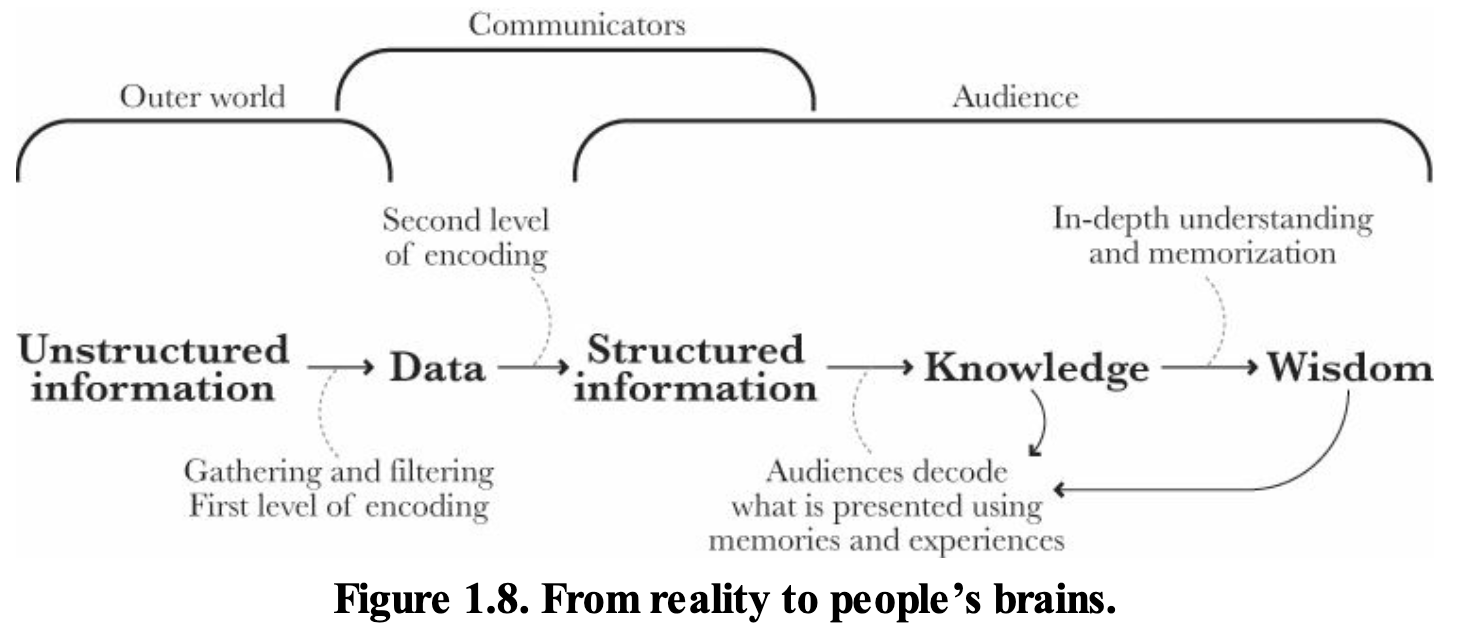
\includegraphics[width=0.95\textwidth]{images/cairo_model.png}
		\caption*{Source is \cite[][page 29]{cairo2012}}
	\end{figure}
\end{frame}

\begin{frame}{How to Navigate the Data Visualization Process?}{}
	\begin{columns}
		\begin{column}{0.5\textwidth}
			\begin{figure}
				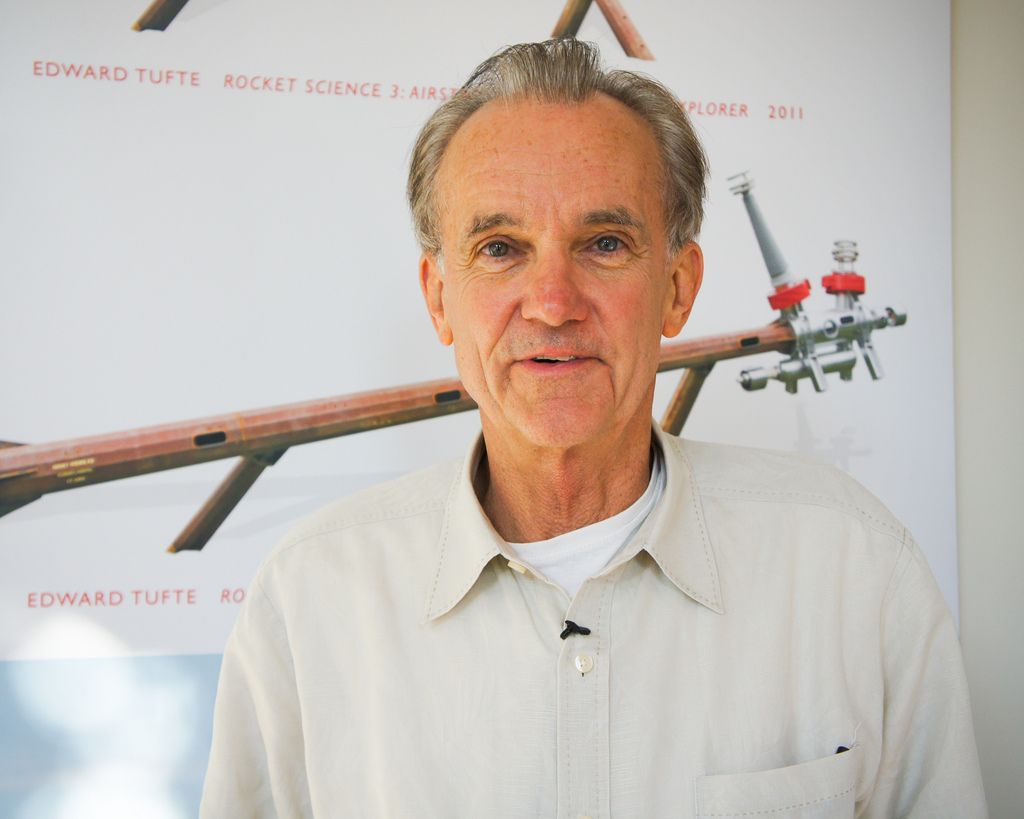
\includegraphics[width=0.95\textwidth]
				{images/edward-tufte.jpeg}
			\end{figure}
		\end{column}
		\begin{column}{0.5\textwidth}
			Tufte \cite[][page 92]{tufte2001} suggests to adhere to a 
			basic design principle:

			\begin{quote}
				\textit{
					Show the data.

					\vspace{2em}
					
					The principle is the basis for a theory,
					for a theory of data graphics.
					}
			\end{quote}
		\end{column}
	\end{columns}
\end{frame}

\begin{frame}{}{}
	\LARGE \centering Fine --- So What?!
\end{frame}

\begin{frame}{Maximize the Data-Ink Ratio!!}{}
	\begin{center}
	\begin{equation*}
		\text{Data-Ink ratio} = \frac{
			\text{data-ink}
			}
			{
			\text{total ink used to print the graphic design}
			}
	\end{equation*}
	\end{center}
	
	\vspace{2em}

	\textbf{Data-ink} is the non-erasable core of a graphic, the 
	non-redundant ink arranged in response to variation in the numbers 
	represented.
\end{frame}

\begin{frame}{John Tukey's Box Plot}{}
	\begin{figure}
		\begin{center}
			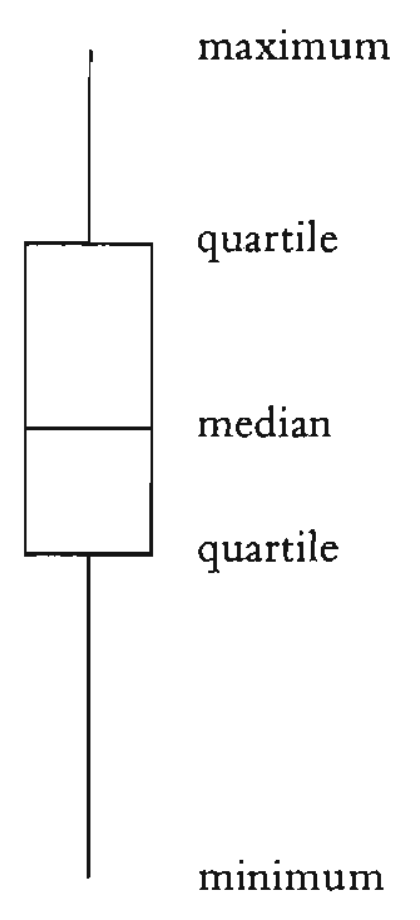
\includegraphics[width=0.25\textwidth]{images/boxplot.png}
		\end{center}
	\end{figure}
\end{frame}

\begin{frame}{A Box Plot with a Limited Data-Ink Ratio}{}
	\begin{figure}
		\begin{center}
			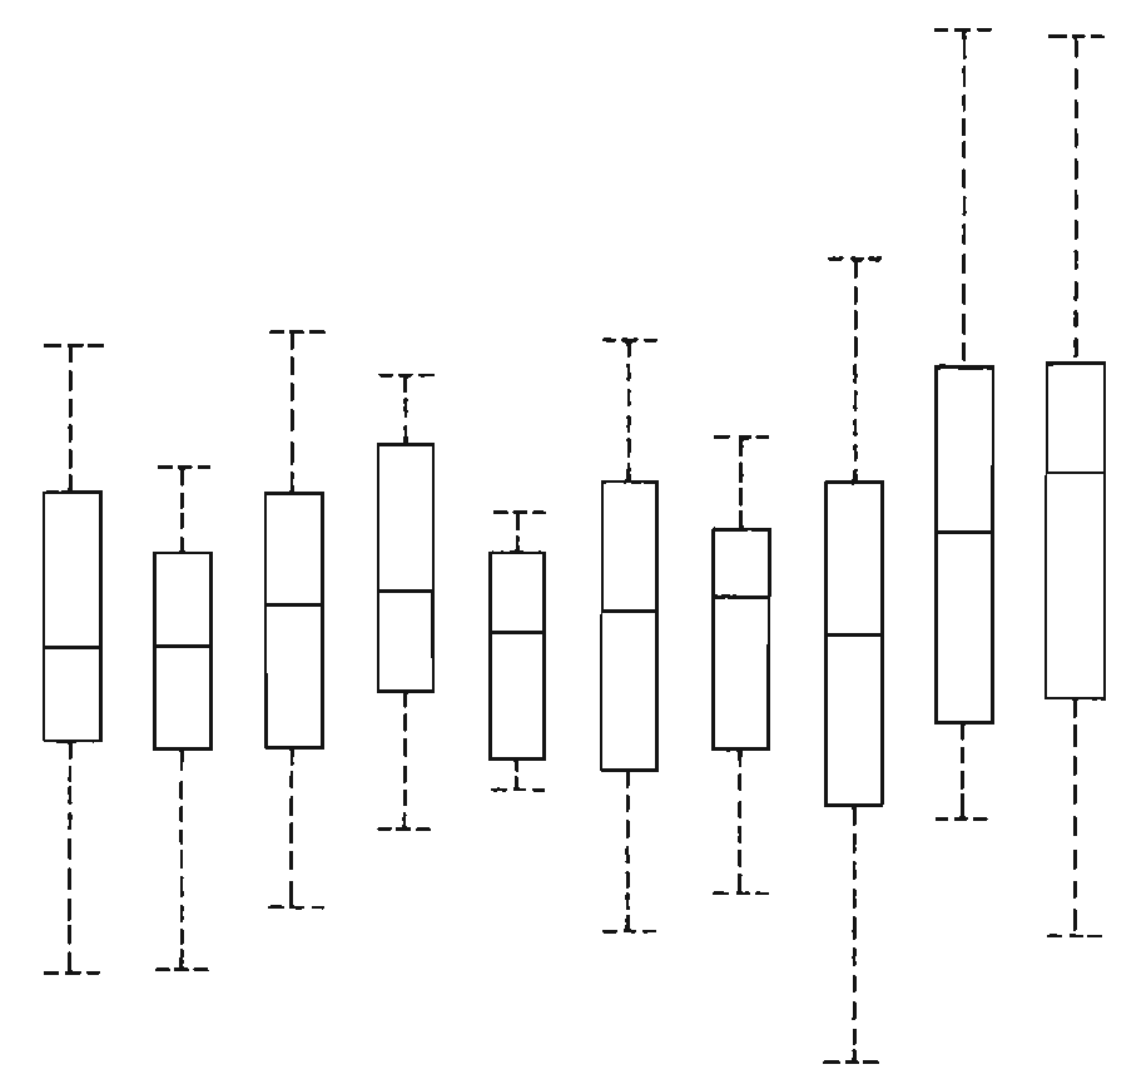
\includegraphics[width=0.6\textwidth]{images/trad_boxplot.png}
		\end{center}
	\end{figure}
\end{frame}

\begin{frame}{Tufte-Alike Box Plot}{}
\begin{figure}
		\begin{center}
			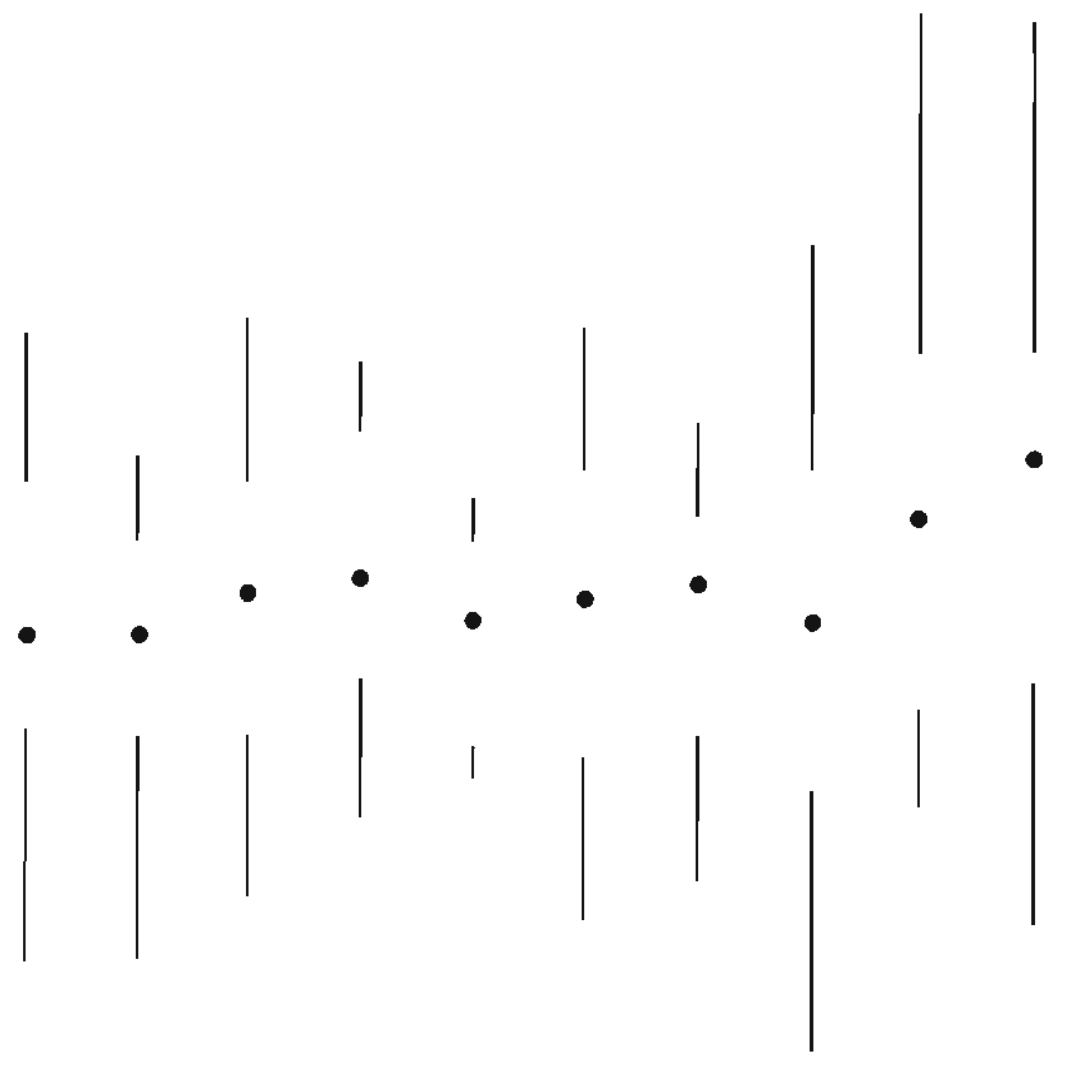
\includegraphics[width=0.6\textwidth]{images/tufte_boxplot.png}
		\end{center}
	\end{figure}

\end{frame}

\begin{frame}{A Bar Chart with a Limited Data-Ink Ratio}{}
\begin{figure}
		\begin{center}
			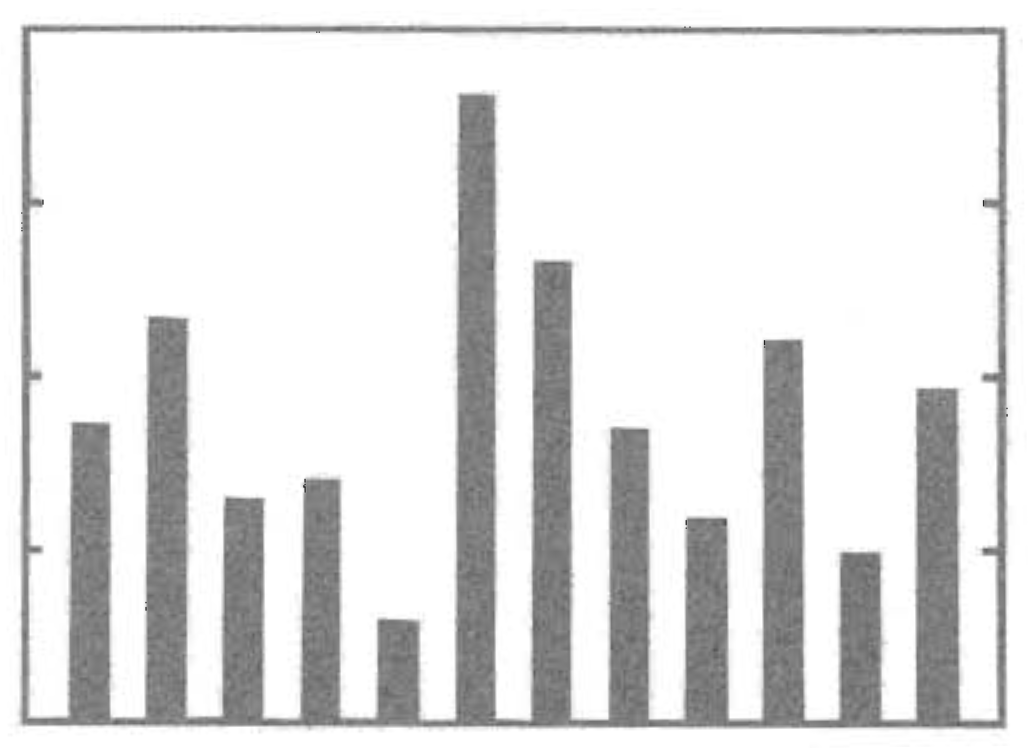
\includegraphics[width=0.75\textwidth]{images/trad_barchart.png}
		\end{center}
	\end{figure}

\end{frame}

\begin{frame}{Tufte-Alike Bar Chart}{}
\begin{figure}
		\begin{center}
			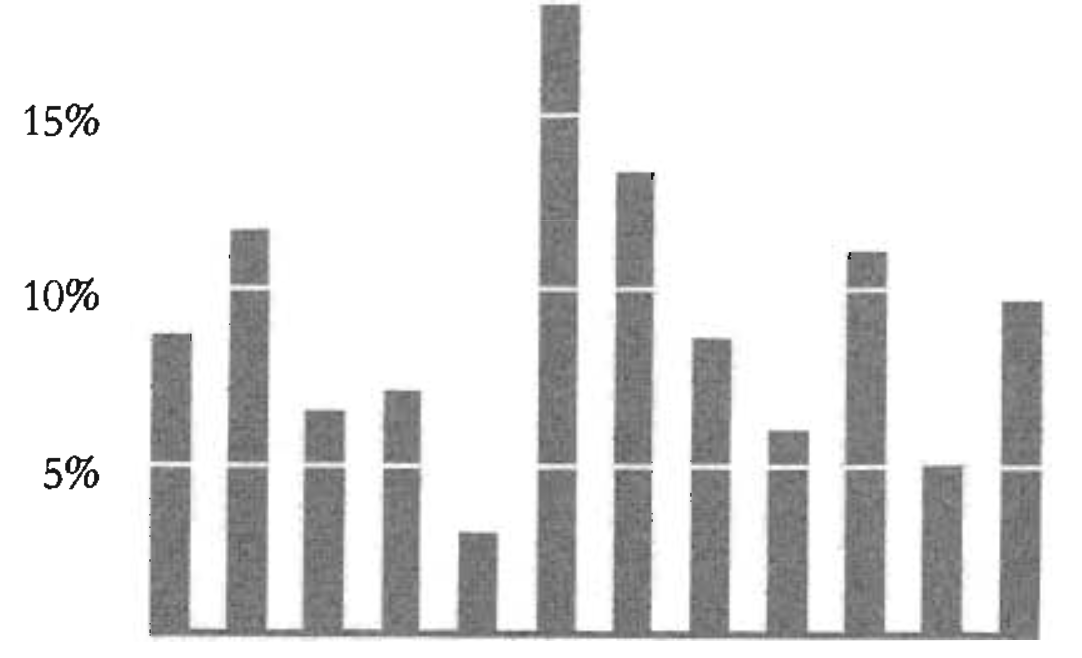
\includegraphics[width=0.8\textwidth]{images/tufte_barchart.png}
		\end{center}
	\end{figure}

\end{frame}

\begin{frame}{A Bare-Bone Scatter Diagram}{}
\begin{figure}
		\begin{center}
			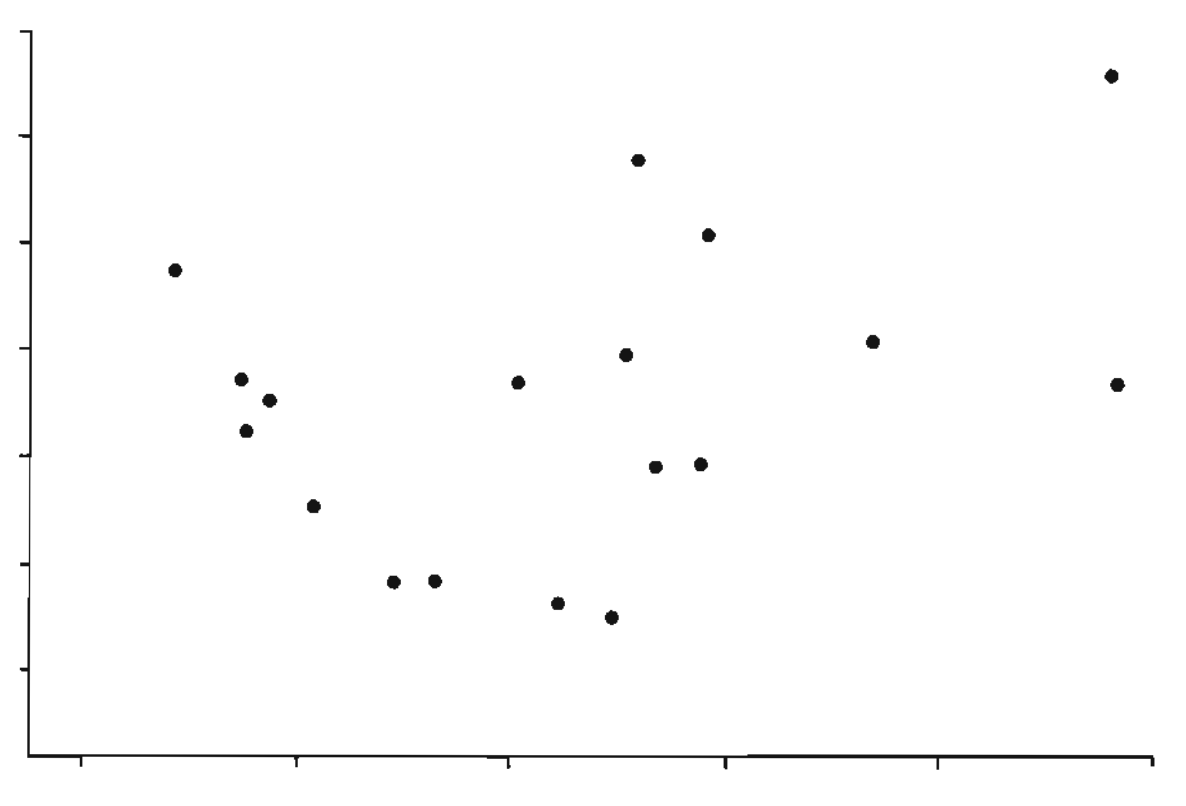
\includegraphics[width=0.8\textwidth]{images/trad_scatter.png}
		\end{center}
	\end{figure}

\end{frame}

\begin{frame}{Tufte-Alike Scatter Diagram}{}
\begin{figure}
		\begin{center}
			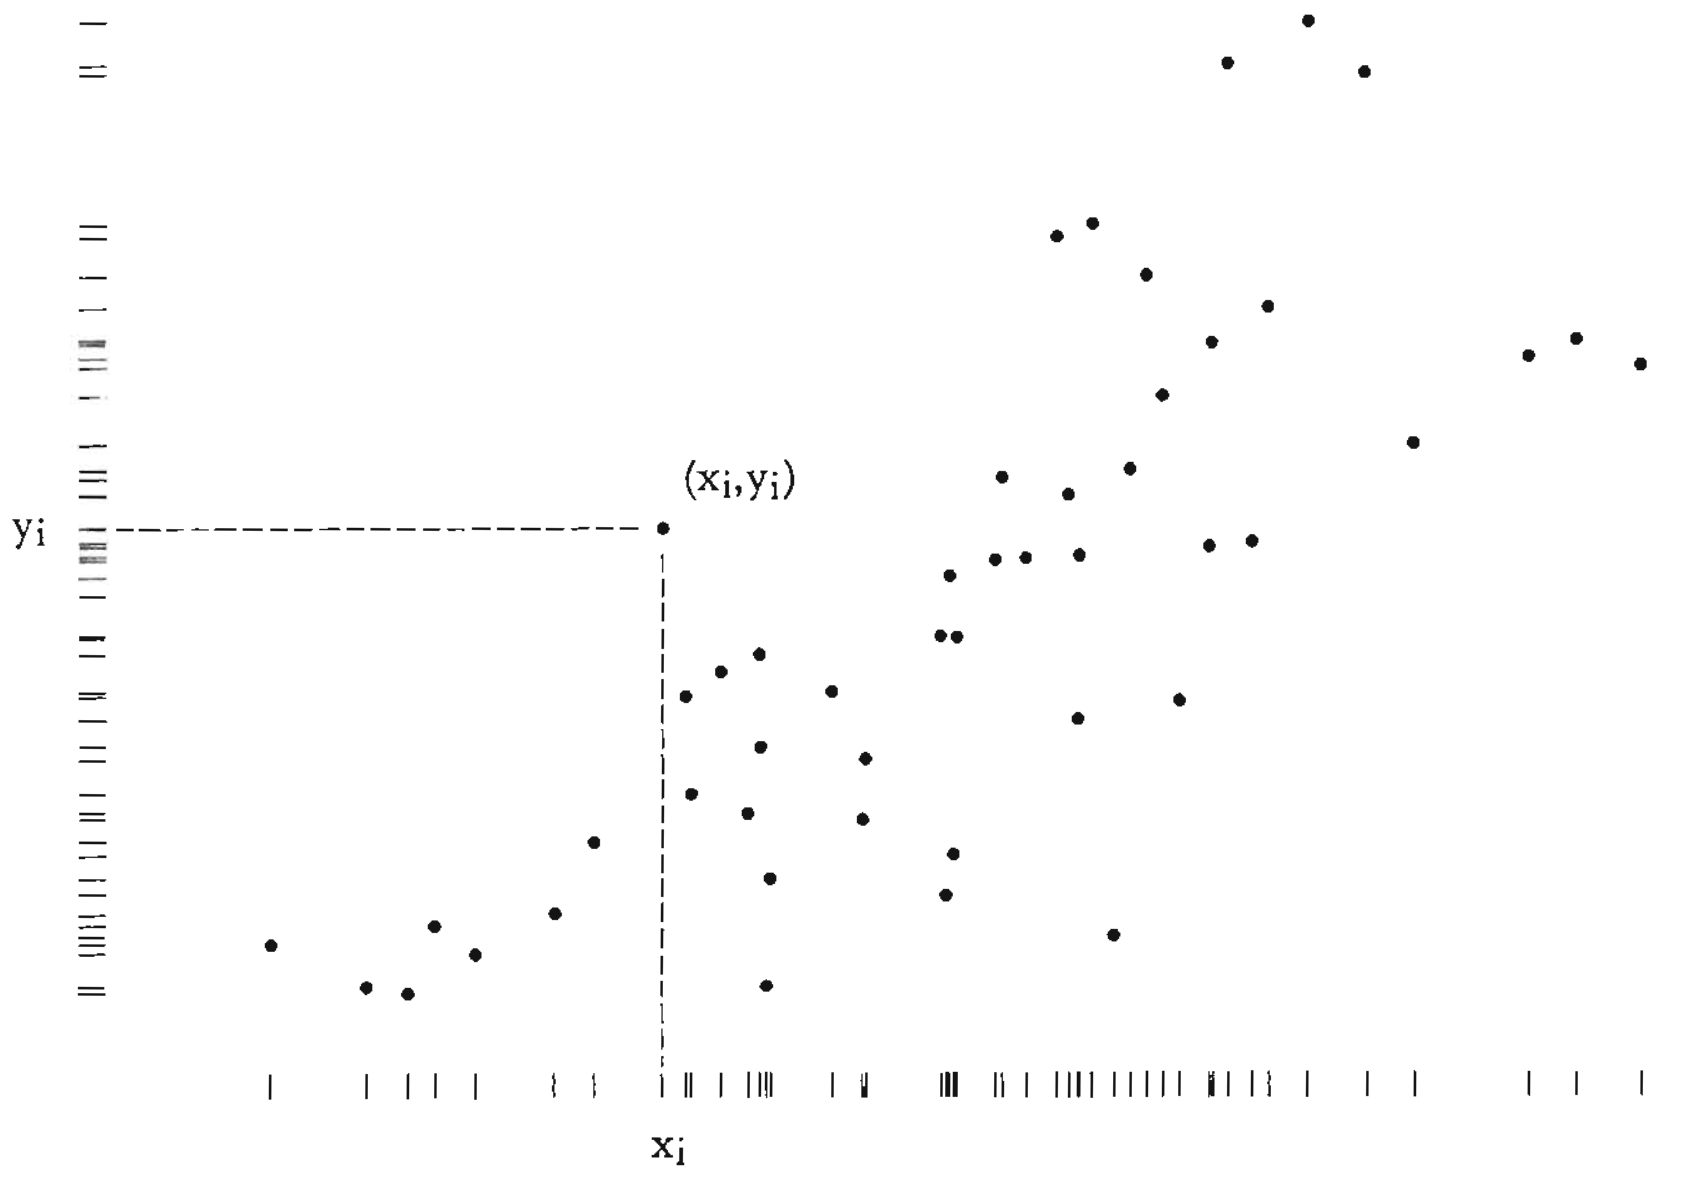
\includegraphics[width=0.85\textwidth]{images/tufte_scatter.png}
		\end{center}
	\end{figure}

\end{frame}

\begin{frame}{Tufte-Alike Scatter Diagram}{}
\begin{figure}
		\begin{center}
			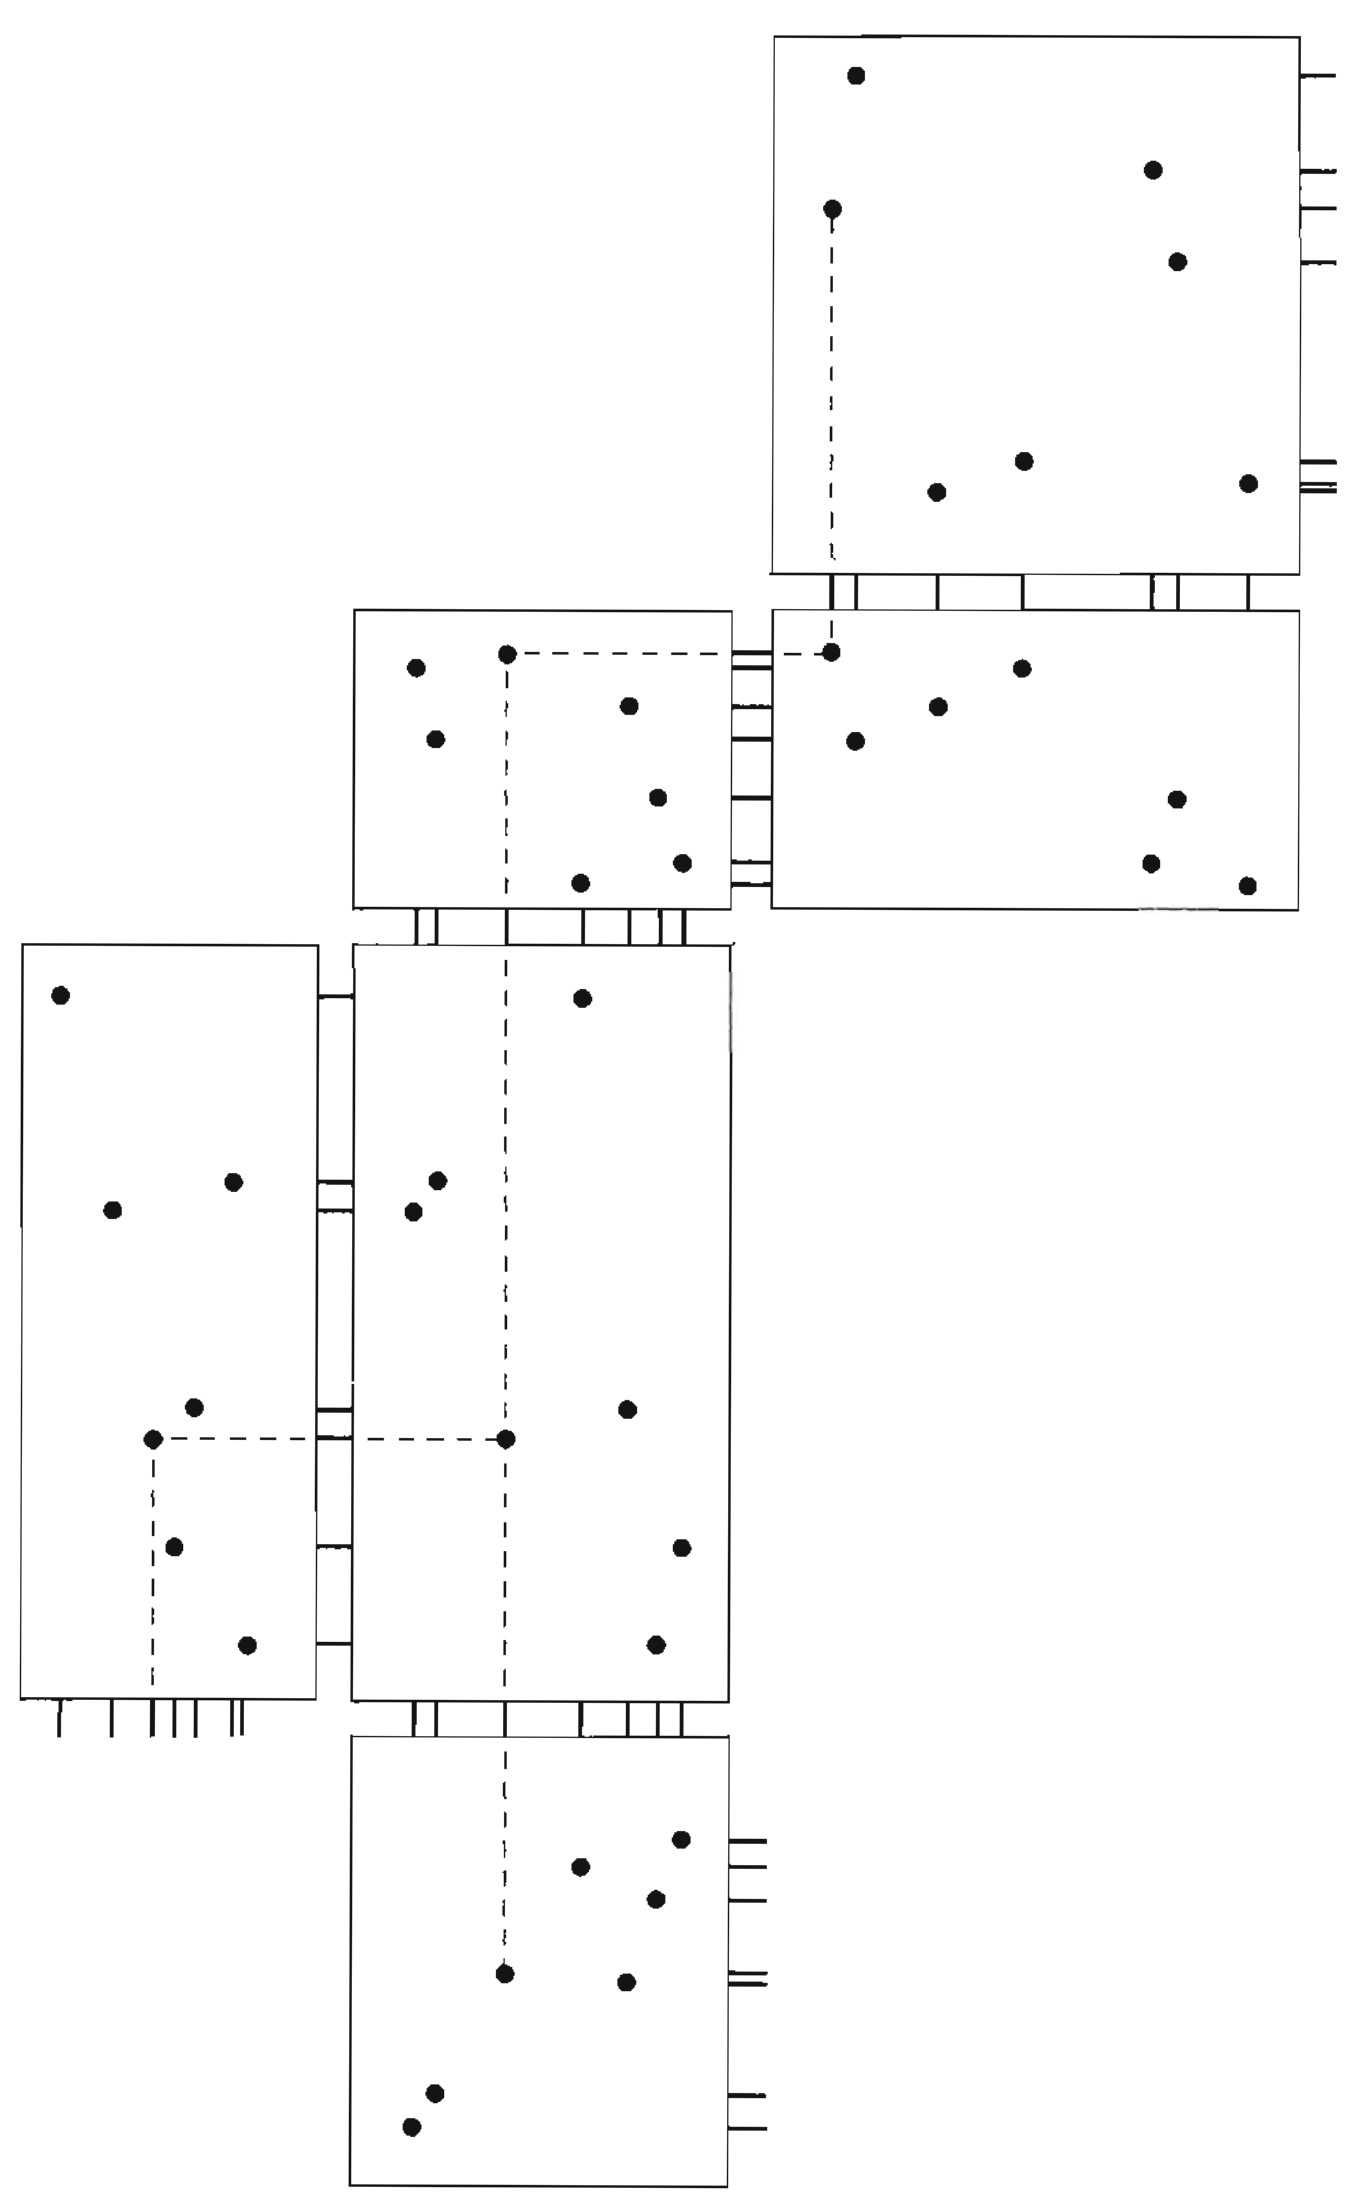
\includegraphics[width=0.35\textwidth]{images/rug_plot.png}
		\end{center}
	\end{figure}
\end{frame}

% ============================= EDA lab ===================================
\section{Exploratory Data Analysis Lab}

\begin{frame}{}{}
	\centering
	\Large How does EDA relate to Cairo's model?
\end{frame}
	

\begin{frame}{The Data Visualization Process according to Cairo}
	{Data, information, knowledge, wisdom}{}
	\begin{figure}
		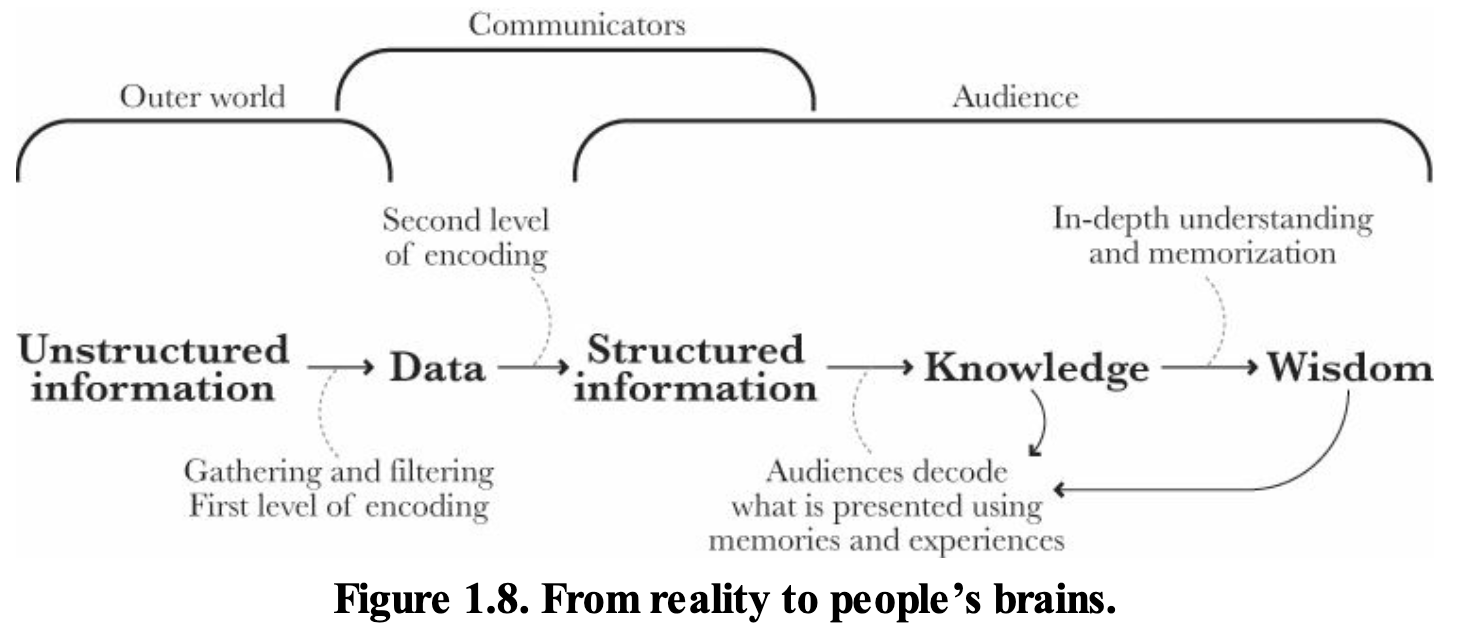
\includegraphics[width=0.95\textwidth]{images/cairo_model.png}
		\caption*{Source is \cite[][page 29]{cairo2012}}
	\end{figure}
\end{frame}

\begin{frame}{}{}
\centering
\Large Time for the Python code and collective discussion!
\end{frame}

% =========================== Graphical perception =========================
\section{Graphical Perception and Color}

\begin{frame}{Let Us Play a Classification Game!}
	{Which outlet does the data visualization come from?}
	\begin{columns}
		\begin{column}{0.25\textwidth}
			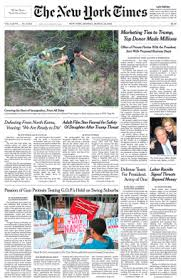
\includegraphics[width=1\textwidth]{images/nyt}
		\end{column}
		\begin{column}{0.23\textwidth}
			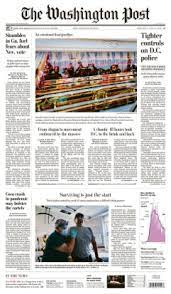
\includegraphics[width=1\textwidth]{images/wp}
		\end{column}
		\begin{column}{0.25\textwidth}
			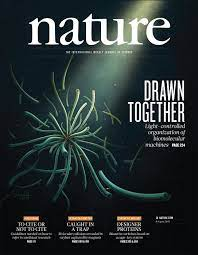
\includegraphics[width=1\textwidth]{images/nature}
		\end{column}
		\begin{column}{0.25\textwidth}
			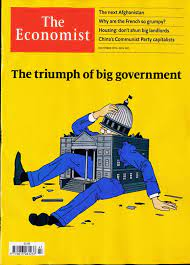
\includegraphics[width=1\textwidth]{images/economist}
		\end{column}
	\end{columns}
\end{frame}

\begin{frame}{?}{}
	\centering
	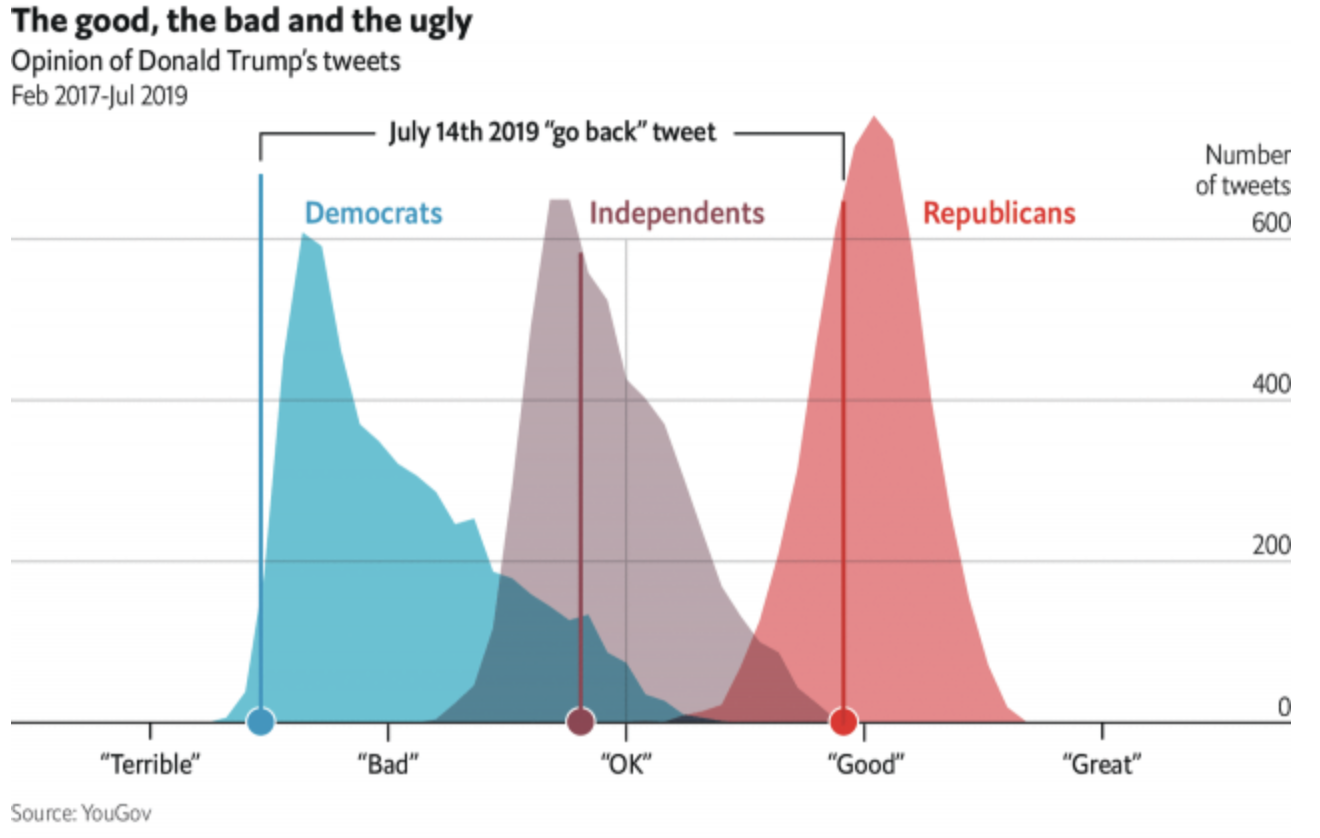
\includegraphics[width=0.8\textwidth]{images/econ_0.png}
	\pause

	The Economist
\end{frame}

\begin{frame}{?}{}
	\centering
	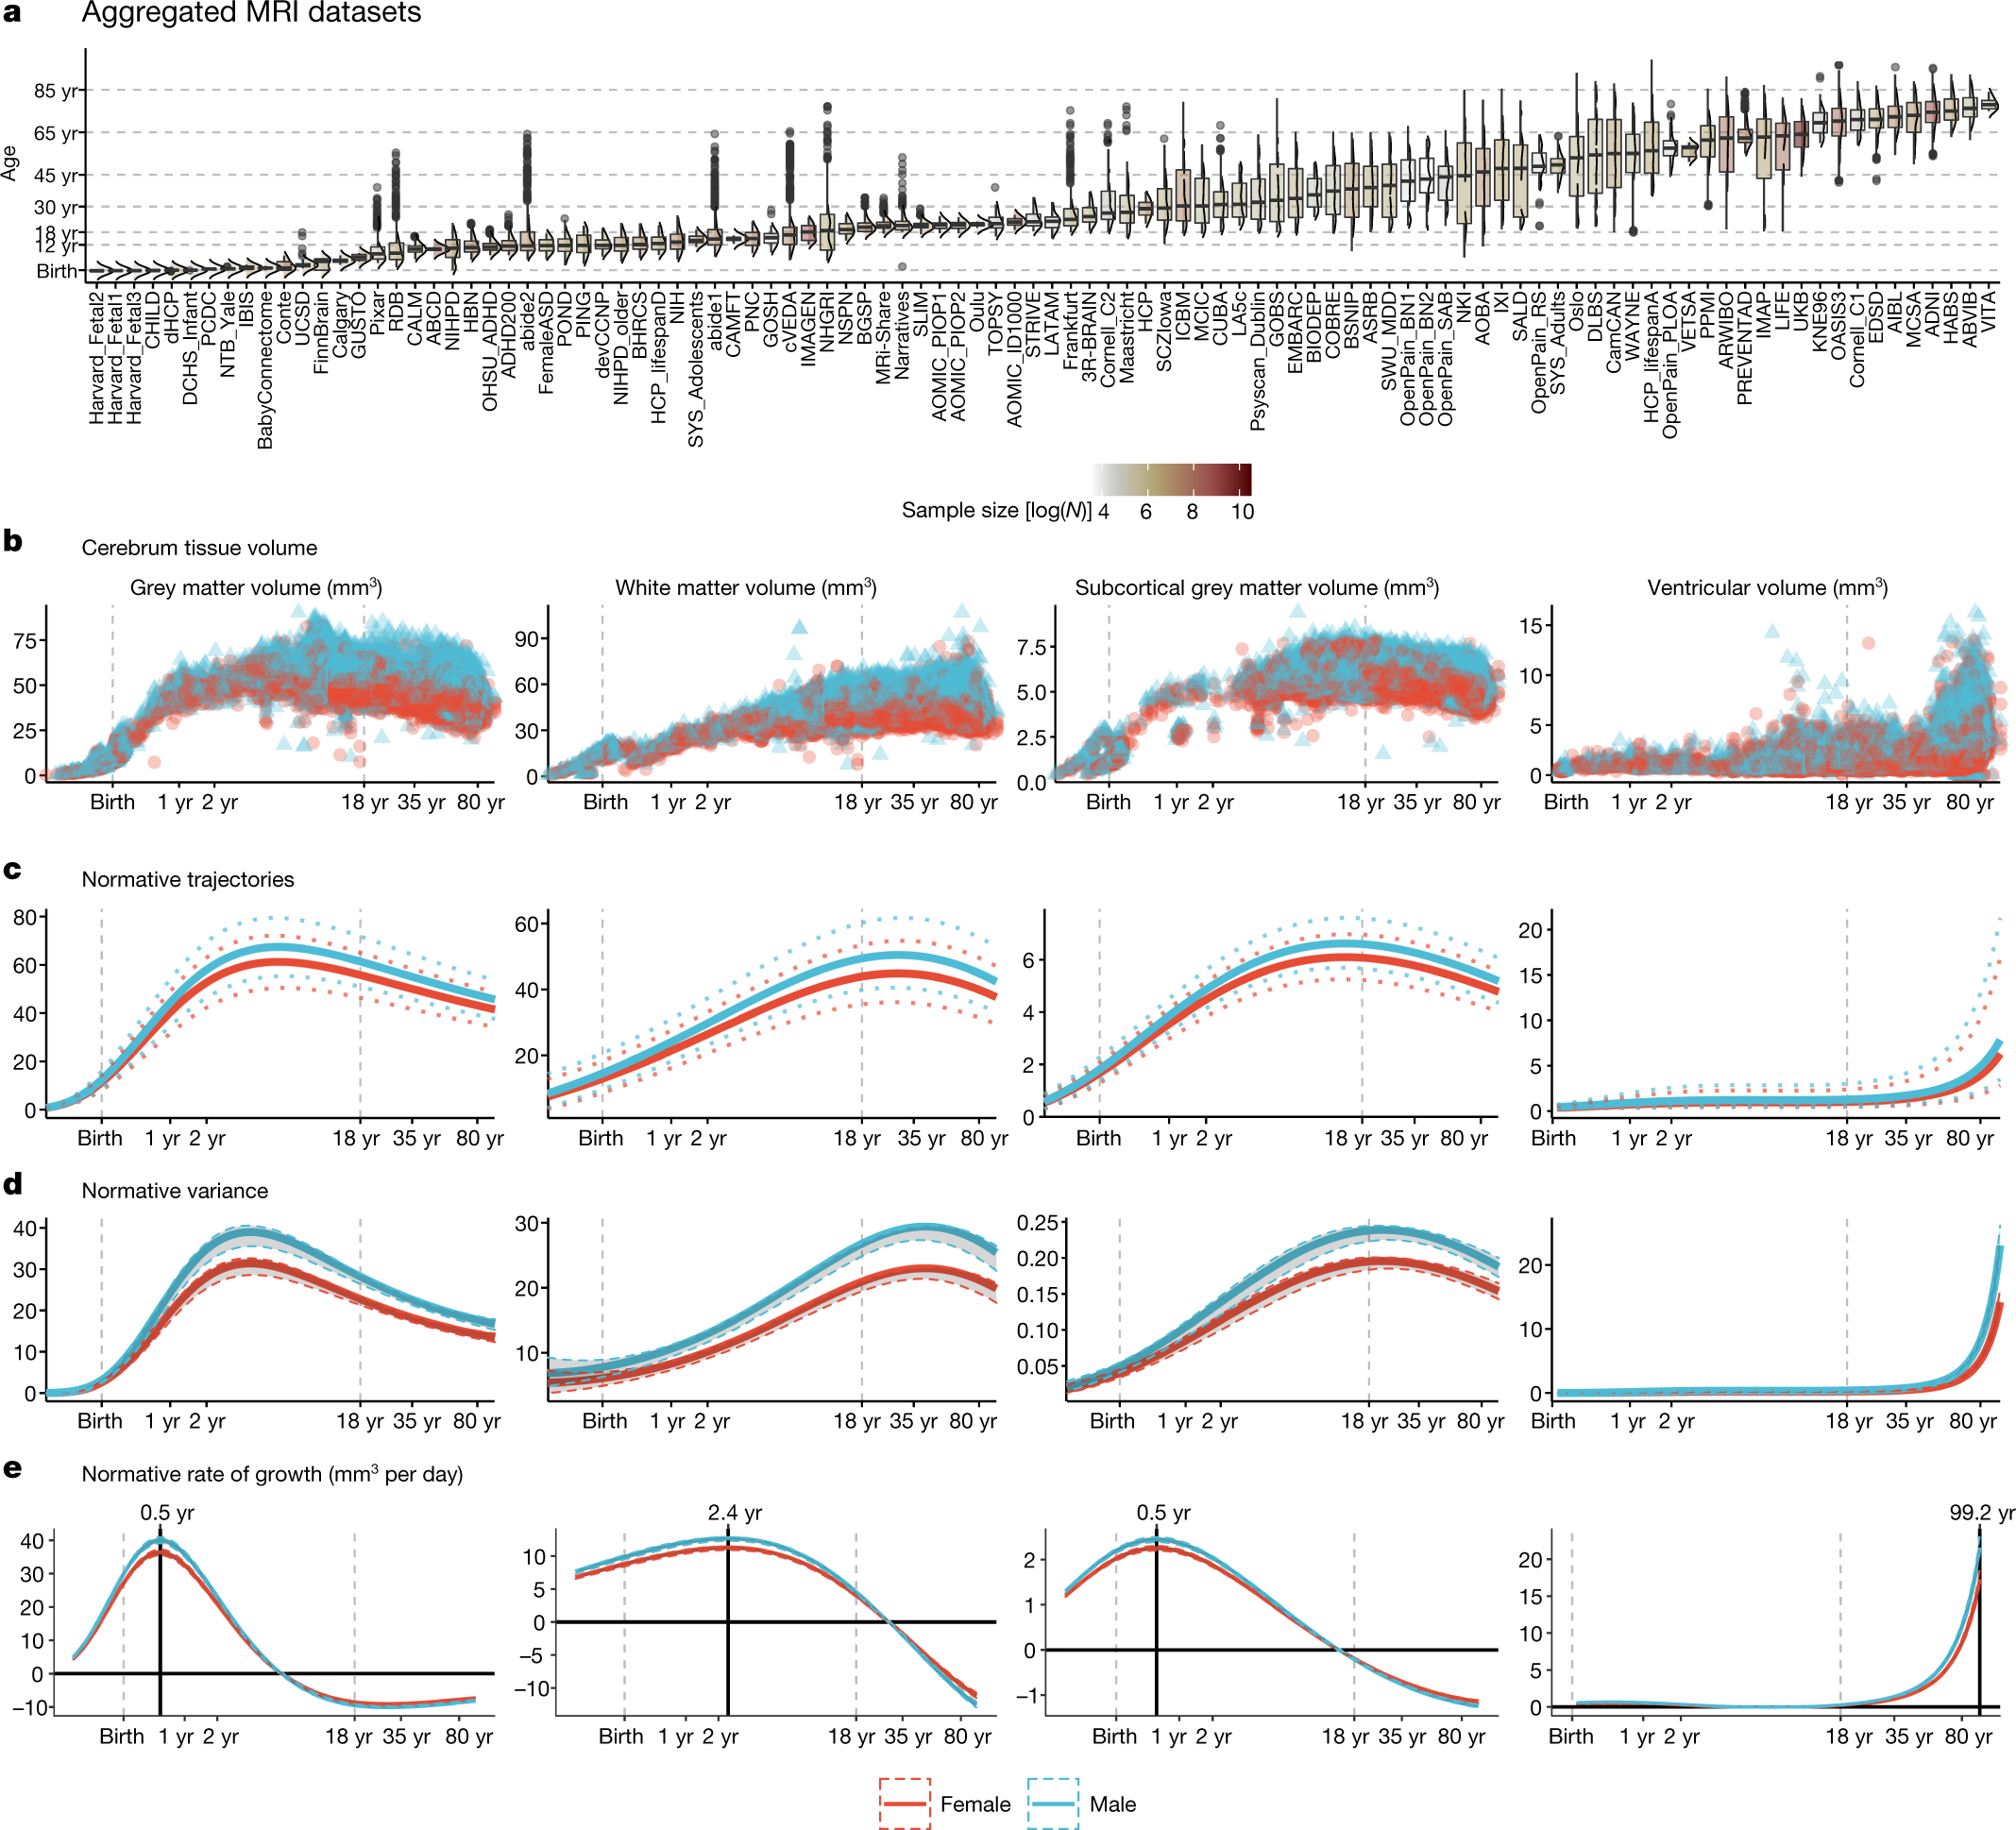
\includegraphics[width=0.6\textwidth]{images/nature_0.png}
	\pause

	Nature
\end{frame}

\begin{frame}{?}{}
	\centering
	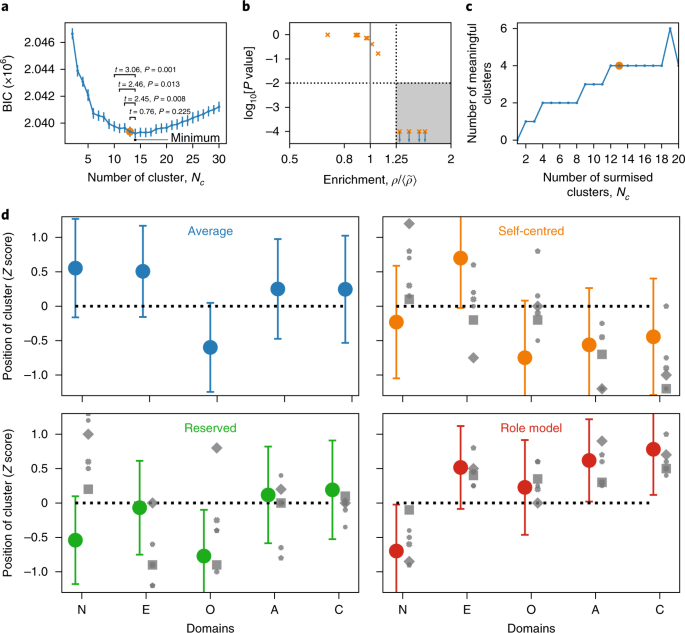
\includegraphics[width=0.6\textwidth]{images/nature_1.png}
	\pause

	Nature
\end{frame}

\begin{frame}{?}{}
	\centering
	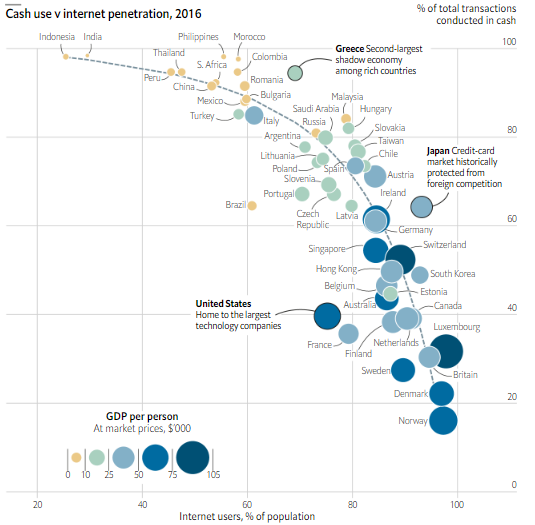
\includegraphics[width=0.55\textwidth]{images/econ_1.png}
	\pause

	The Economist
\end{frame}

\begin{frame}{?}{}
	\centering
	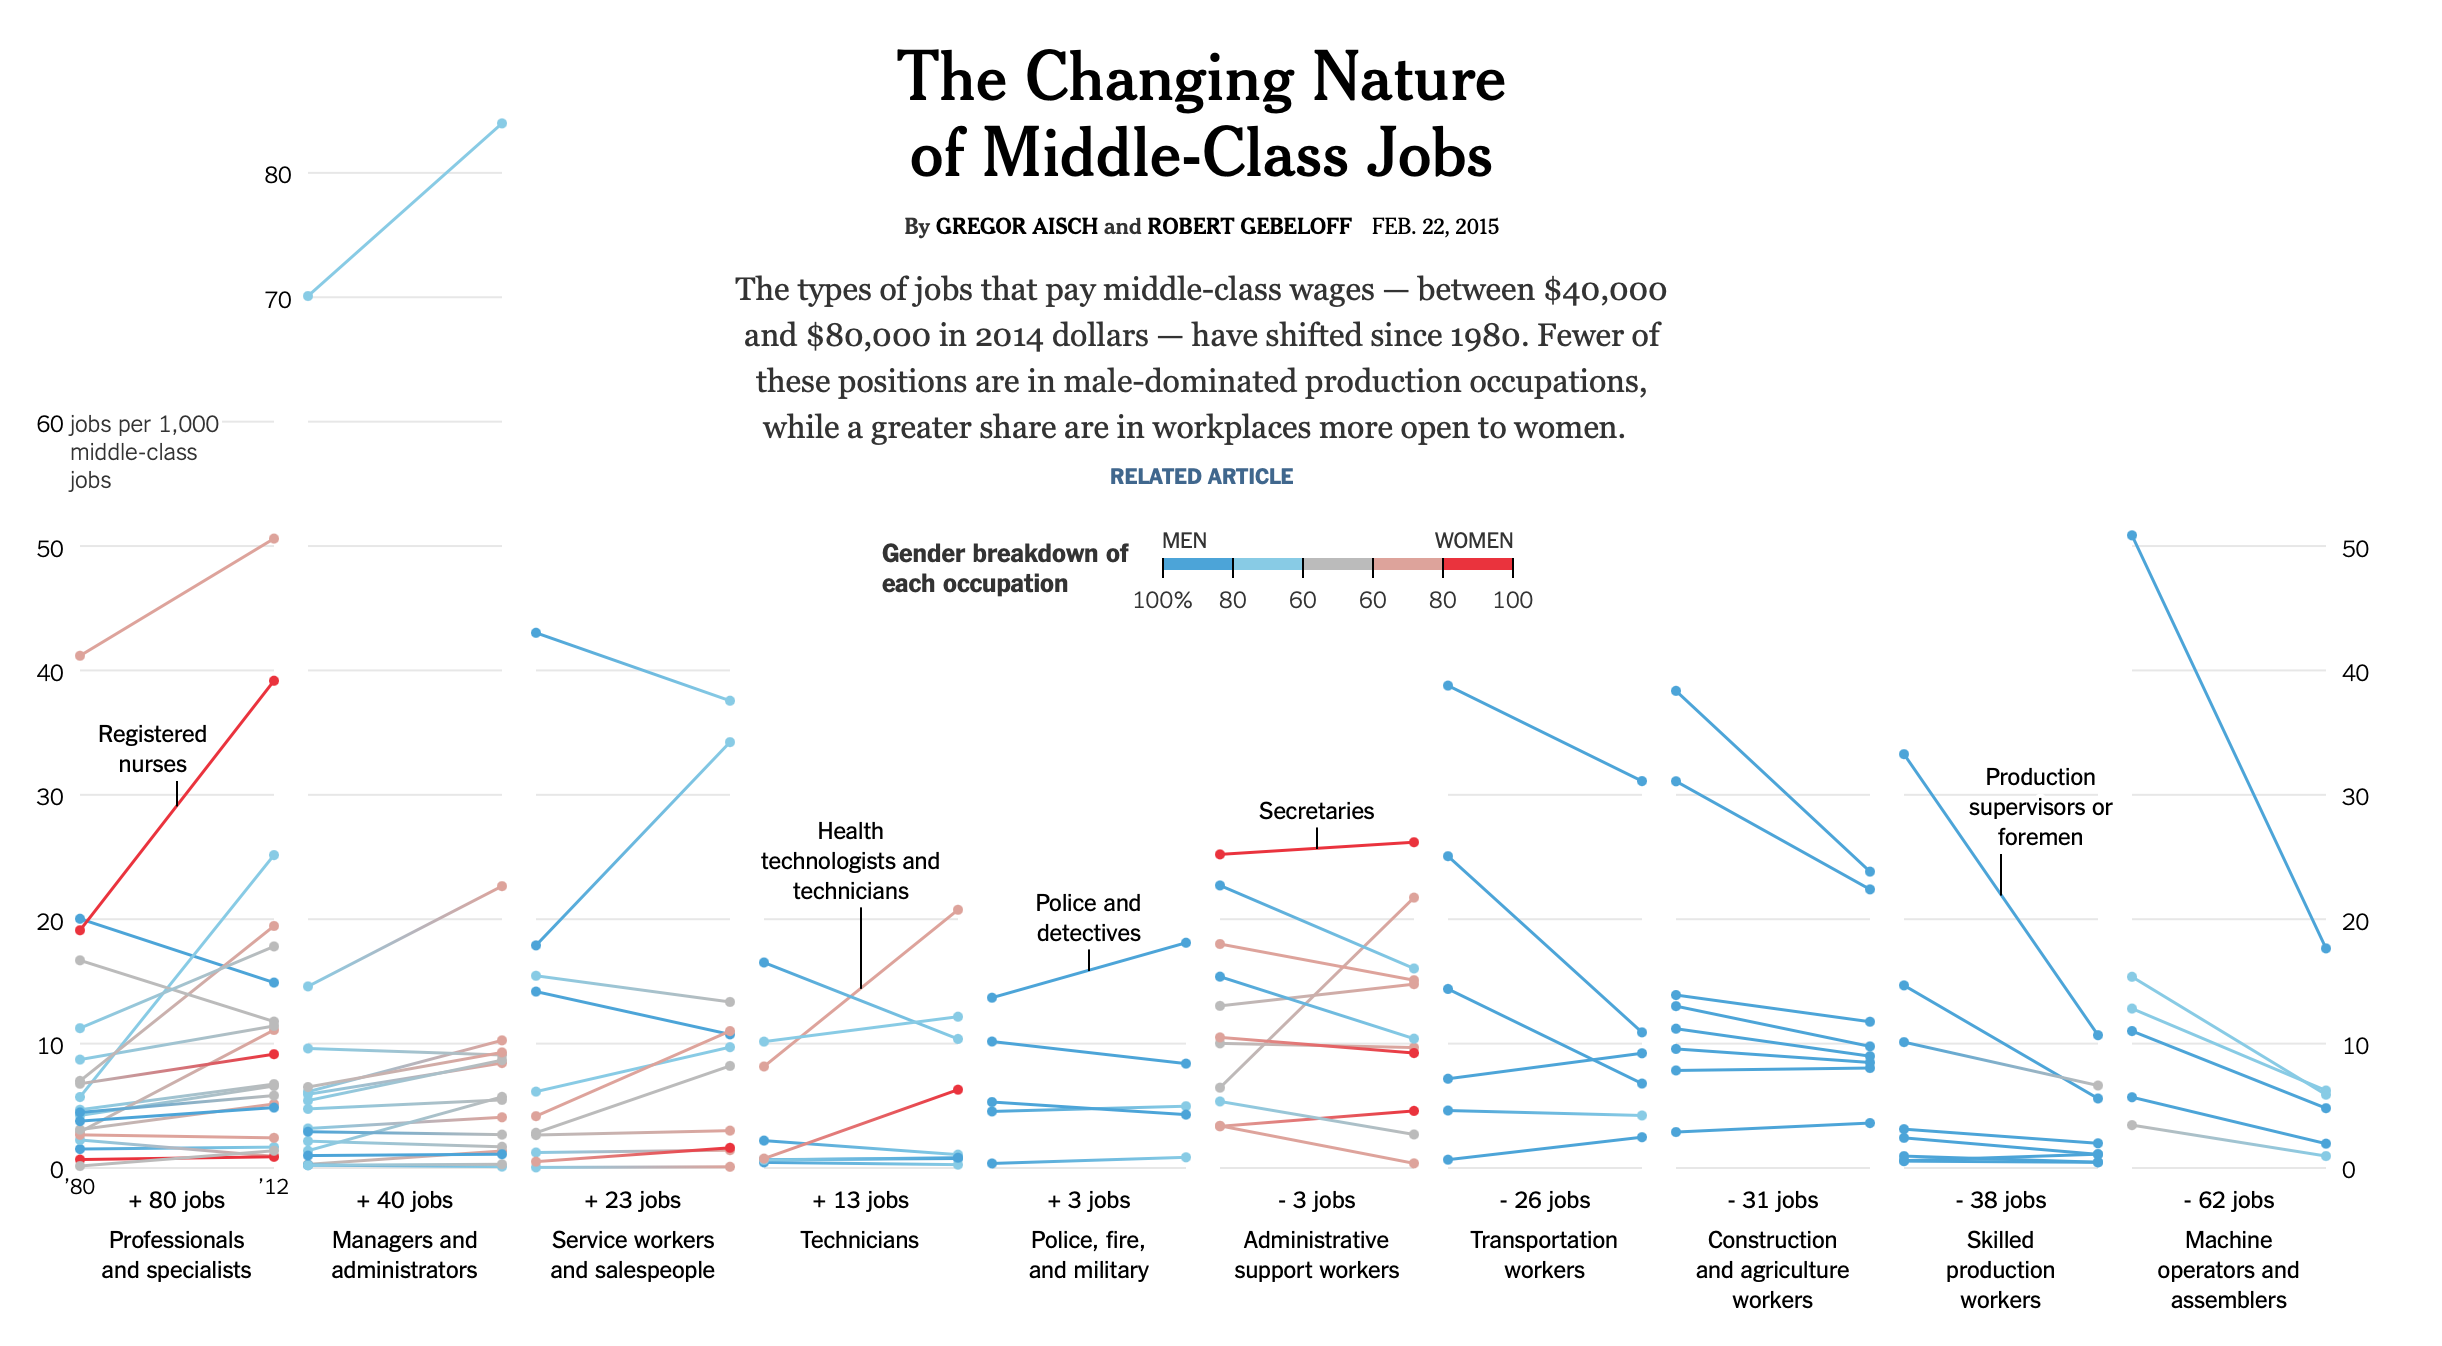
\includegraphics[width=0.9\textwidth]{images/nyt_0.png}
	\pause

	NYT
\end{frame}


\begin{frame}{?}{}
	\centering
	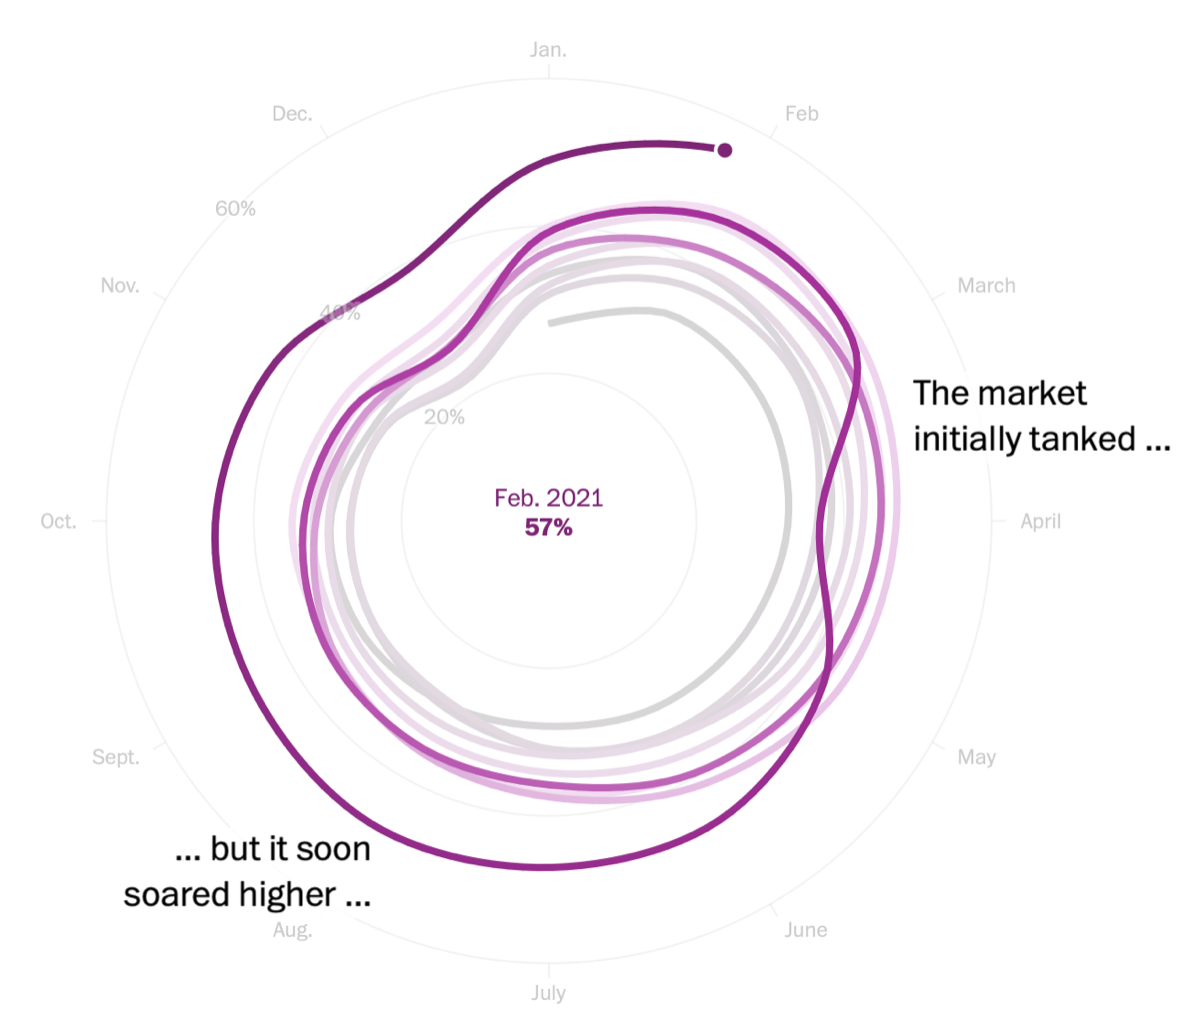
\includegraphics[width=0.6\textwidth]{images/wp_0.png}
	\pause

	Washington Post
\end{frame}


\begin{frame}{?}{}
	\centering
	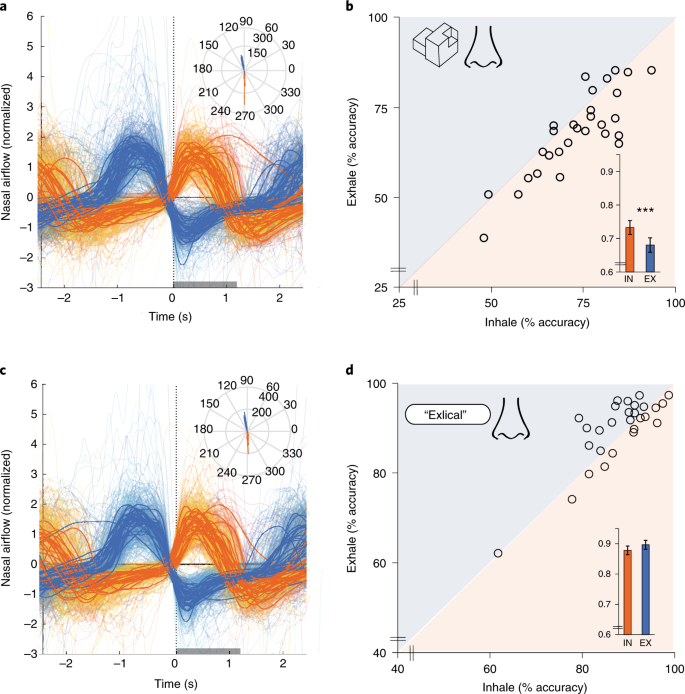
\includegraphics[width=0.5\textwidth]{images/nature_2.png}
	\pause

	Nature
\end{frame}

\begin{frame}{}{}
	\centering
	\Large What is the take-home message from the comparison of different
	data viz examples?
\end{frame}

\begin{frame}{Designing the `Lower-Level' Features of a Chart}
	{Source \cite[][page 61]{cairo2012}}
	\centering 
	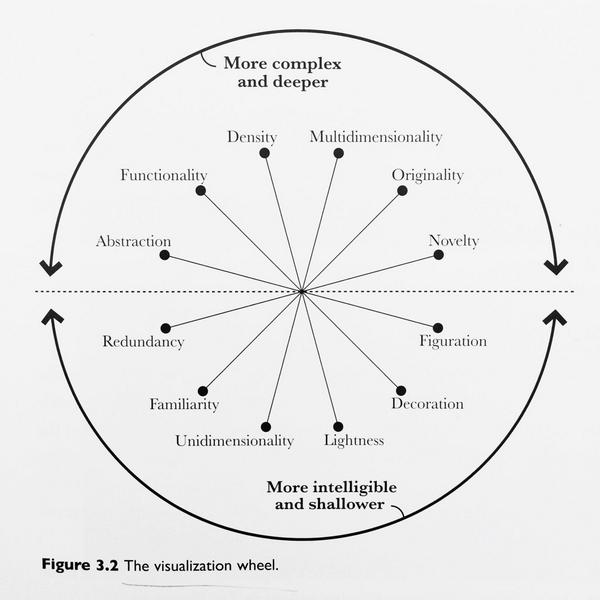
\includegraphics[width=0.55\textwidth]{images/viz_wheel.jpeg}
\end{frame}

\begin{frame}{Designing the `Lower-Level' Features of a Chart}
	{Source \cite[][page 63]{cairo2012}}
	\centering 
	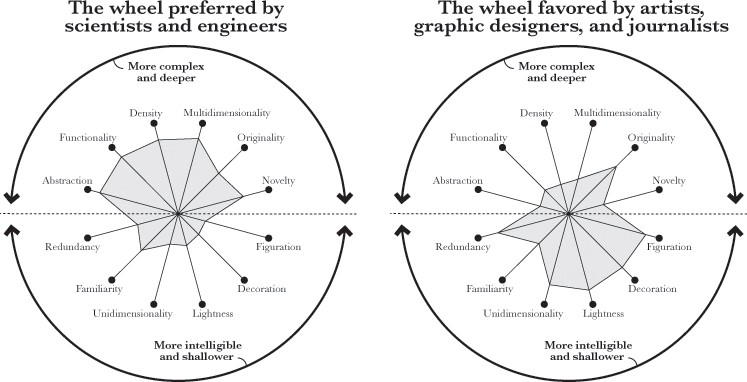
\includegraphics[width=0.9\textwidth]{images/viz_whell_comparison.jpeg}
\end{frame}

\begin{frame}{Chartjunk?}{}
	\centering 
	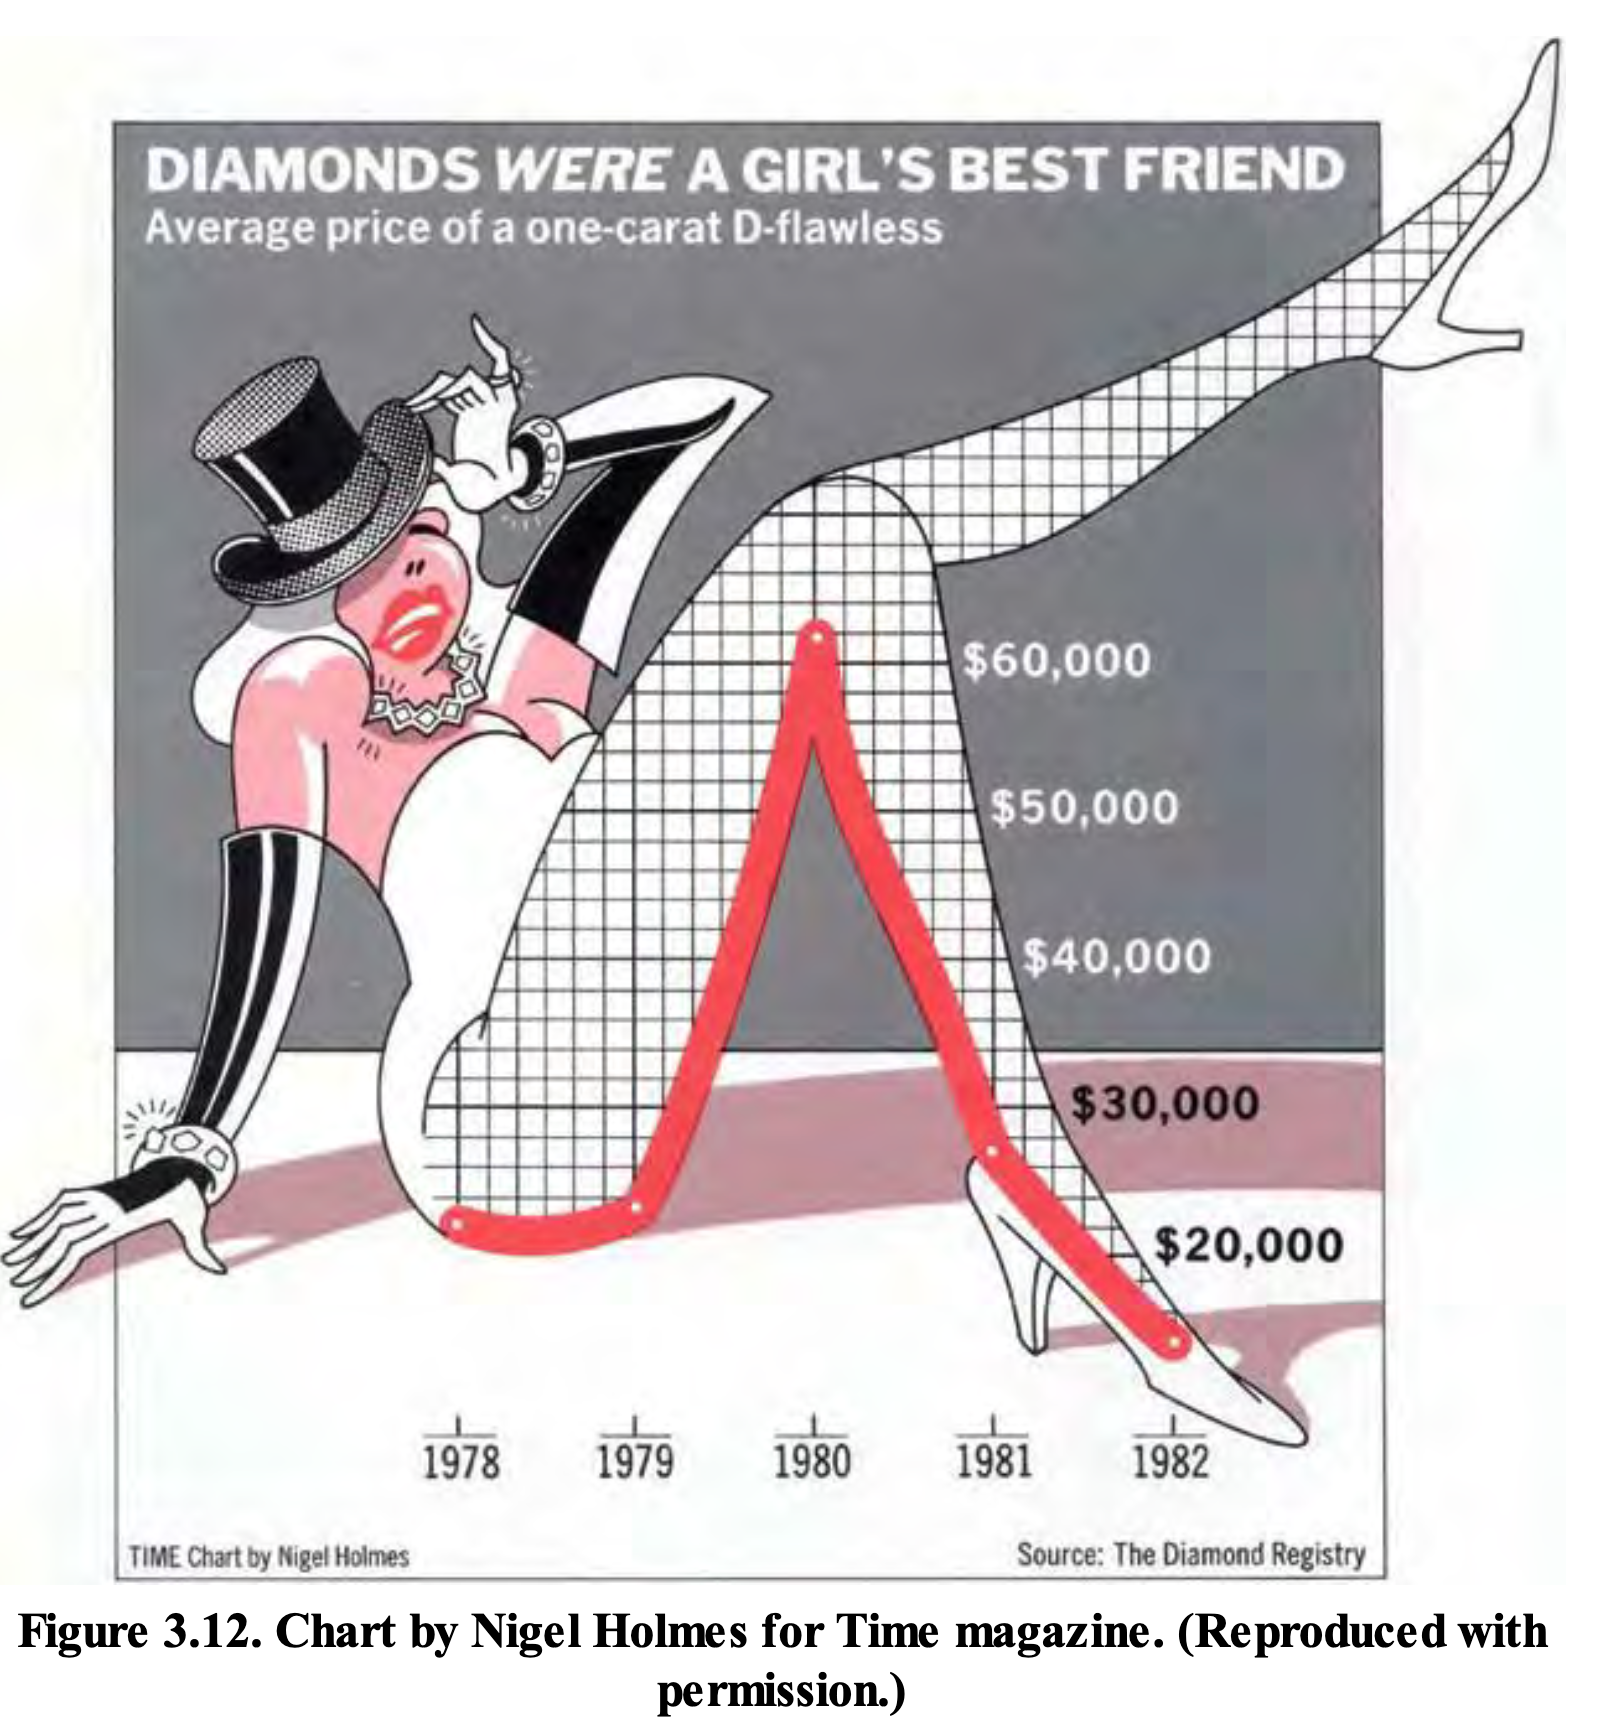
\includegraphics[width=0.55\textwidth]{images/chartjunk.png}
\end{frame}

\begin{frame}{Chartjunk or Memorable?}{}
	\centering 
	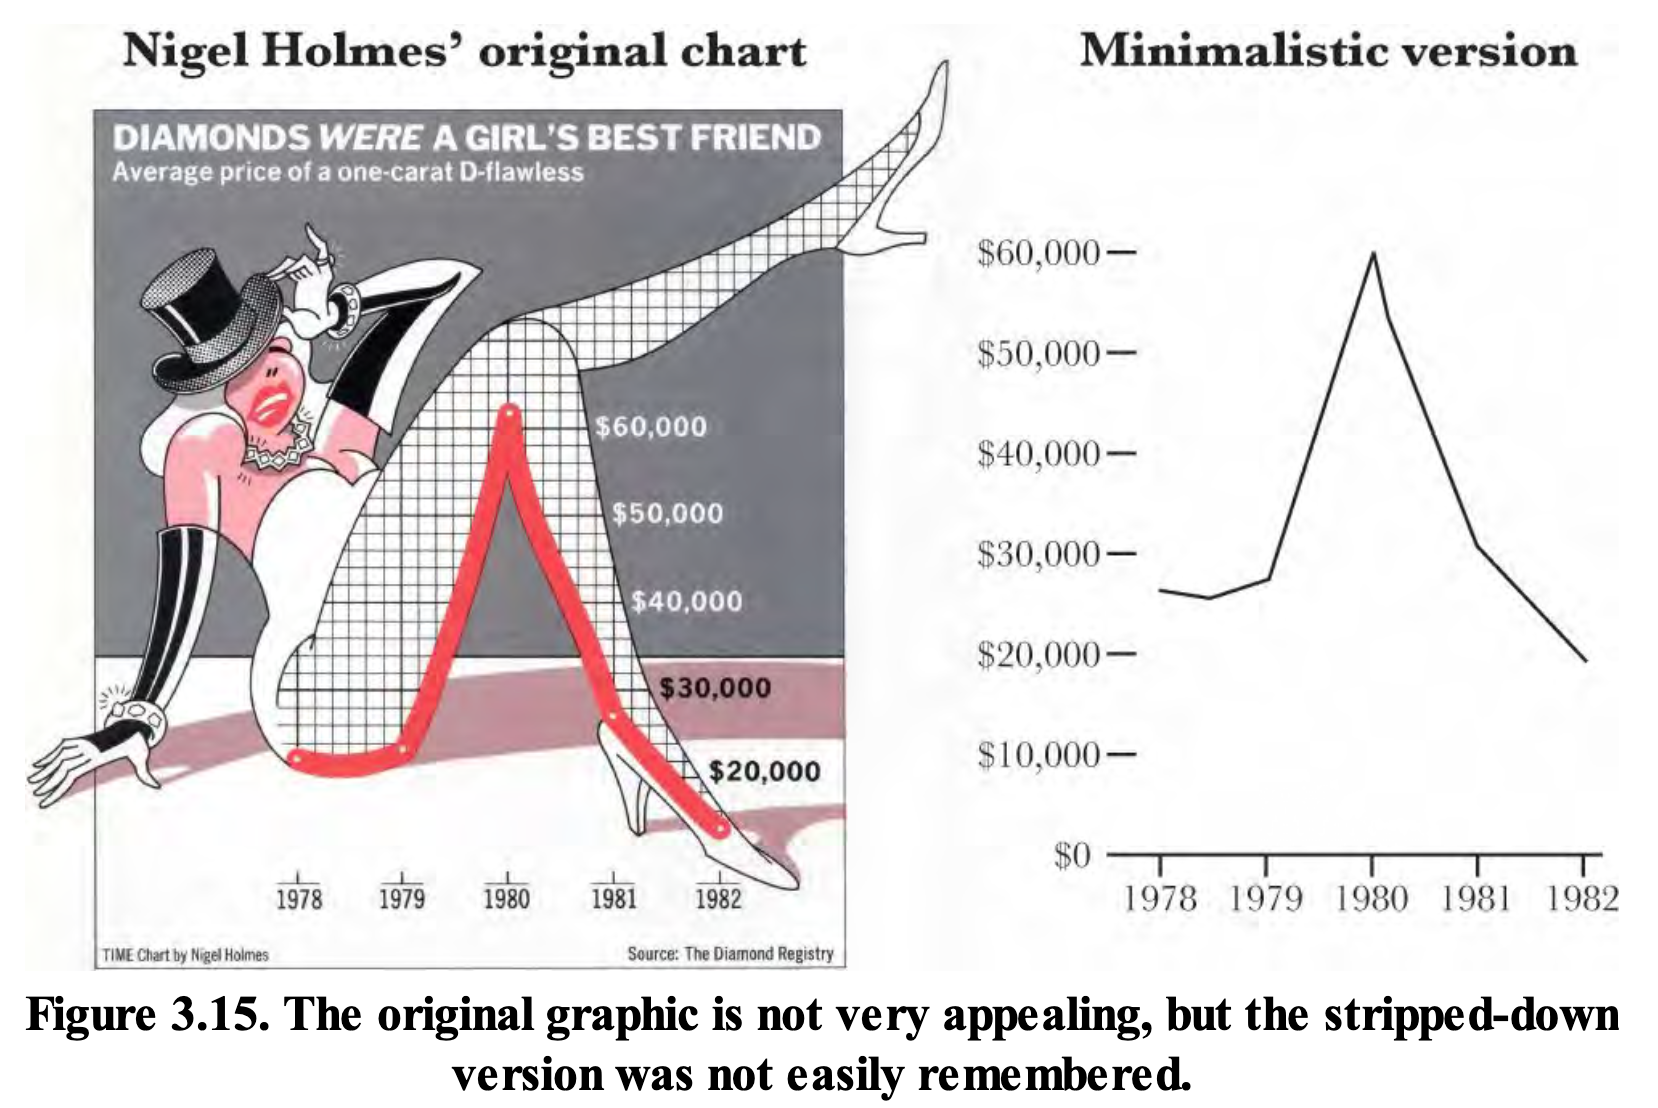
\includegraphics[width=0.8\textwidth]{images/chartjunk_vs_tufter.png}
\end{frame}

\begin{frame}{}{}
	\centering
	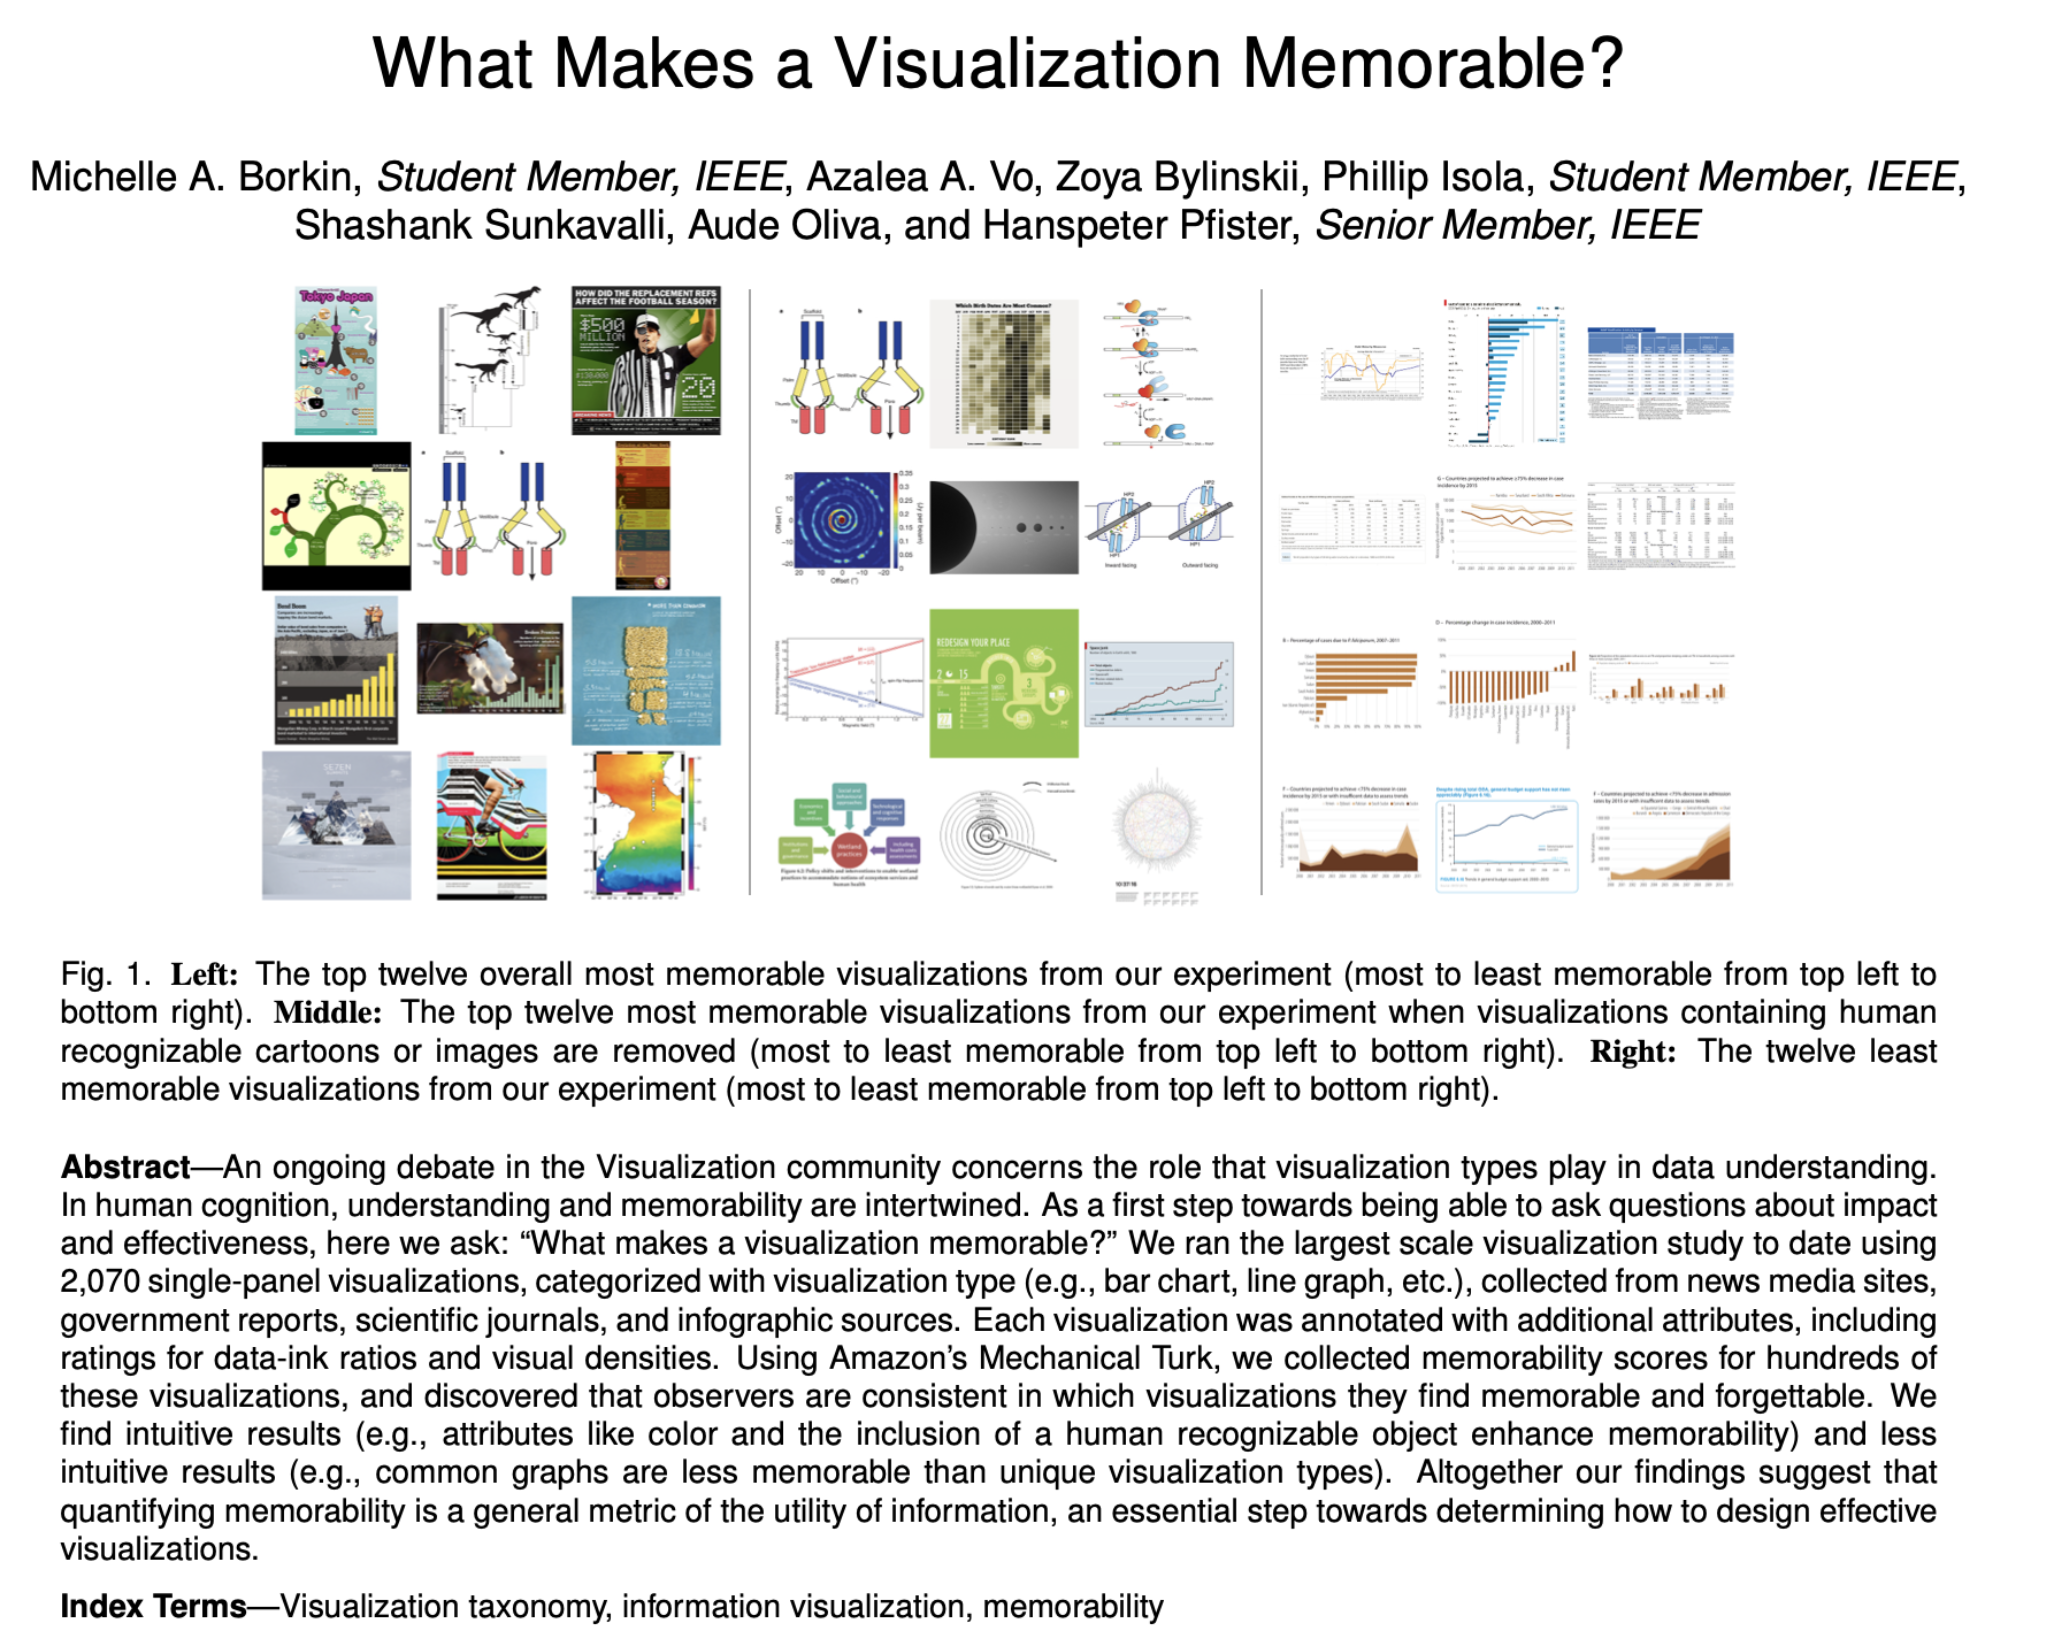
\includegraphics[width=0.7\textwidth]{images/memorable_data_viz.png}
\end{frame}

% ========================== Session 4 wrap up =============================
\section{Session \#4 Wrap Up}

\begin{frame}{}{}
	\LARGE \centering Time to wrap up!
\end{frame}

% =========================== Bibliography =================================
\begin{frame}
	\frametitle{References}
	\printbibliography
 \end{frame} 

\end{document}